%!TEX root = Thesis.tex

\section{Driving \& Dissipation}
We now introduce a driving term into the Jaynes Cummings Hamiltonian. It is added coherently i.e. the system evolves unitarily with the drive, rather than the more general incoherent case \cite{Xu2014}, and the Hamiltonian reads:
\begin{equation}
  \ham_{JC} = \hbar \omega_d \cre \ann + \hbar \omega_q \atann \atcre +\hbar g (\cre \atann+ \hat{a} \atcre) + \hbar \Epsilon (\cre e^{i\omega_d t} + \ann e^{-i\omega_d t})
\end{equation}
We also consider the effect of dissipation via two collapse operators, the spontaneous decay of the atom via $\atann$, with strength $\gamma$ and the decay of the cavity field via $\ann$, with strength $\kappa$. The total master equation reads:
\begin{equation}
  \dot{\rho} = \frac{1}{i\hbar}[\ham_{JC}, \rho] + \mathscr{L}_\kappa[\rho] + \mathscr{L}_\gamma[\rho]
\end{equation}
We first move to a frame rotating at the drive frequency, giving a hamiltonian:
\begin{equation}
  \ham = \delta_{qd} \cre \ann + \delta_{cd} \atcre \atann + \hbar (\cre \atann + \ann \atcre) + \hbar (\ann + \cre)
\end{equation}
where the explicit time dependence has been removed.
where $\mathscr{L}$ represents the Lindblad dissipator for each collapse parameter

\subsection{Photon Blockade}
With the cavity field on resonance ($\delta_{cd} = \delta_{cd} = \Delta$) with the two level transition, and for now neglecting the drive, the Jaynes Cummings Hamiltonian can be written \cite{Carmichael2015}
\begin{equation}
  \ham_{JC} = \hbar \Delta (\cre \ann + \atann \atcre) +\hbar g (\cre \atann + \hat{a} \atcre)
\end{equation}
Diagonalising yields the \emph{dressed states}
\begin{align}
  \ket{E_{n, U}} & = \frac{1}{\sqrt{2}} (\kettens{n}{-}+\kettens{n-1}{+}) \\
  \ket{E_{n, L}} & = \frac{1}{\sqrt{2}} (\kettens{n}{-}-\kettens{n-1}{+})
\end{align}
in the tensor product of the field fock space and the atomic eigenspace spanned by the bare eigenstates $\ket{+}, \ket{-}$. These dressed eigenstates are superpositions of the bare states $\kettens{n}{-}$ and $\kettens{n-1}{+}$ and are balanced only in the resonant case. The eigenenergies are
\begin{align}
  E_{n, U} &= n \hbar \omega_0 + \sqrt{n} \hbar g \\
  E_{n, L} &= n \hbar \omega_0 - \sqrt{n} \hbar g
\end{align}
in which the Rabi splitting between the upper and lower dressed states is clear. In the absence of coupling to a dressing field $(g=0)$ the Jaynes-Cumming energies form a degenerate harmonic ladder; it is clear that the qubit coupling induces an anharmonicity via the characteristic $\sqrt{n}$ Rabi splitting.

We now consider the effect of an external drive tuned to the $\ket{G} \rightarrow \ket{E_{1, U/L}}$ transition\footnote{Drive frequencies at multiphoton resonances induce the same effect} (where $\ket{G}$ is the coincident dressed ground state $\ket{E_{0, -}} = \kettens{0}{-}$) with frequency $\omega_D = \hbar \omega_0 \pm \hbar g$.
The $\kettens{1}{U/L} \rightarrow \kettens{2}{U/L}$ step of the Jaynes Cummings ladder is now detuned from the drive by $E_{2, U/L} - E_{1, U/L} - \hbar \omega_D =  \mp(2-\sqrt{2}) \hbar g$. Thus for sufficiently large g and sufficiently small linewidth, the upper steps of the ladder are inaccessible, and the Jaynes Cumming system is opaque to further photon absorption until the photon is reemitted from the cavity through some loss process. This is the photon blockade effect.
\subsubsection{Large n detuning approximation}\cite{Alsing1990}
Given a driving field as above, the upper and lower path rungs (n, n+1, \dots) will be detuned from resonant drive by
\begin{align}
  \Delta E_u = \hbar g (\sqrt{n}-\sqrt{n-1}) \\
  \Delta E_l = -\hbar g (\sqrt{n}-\sqrt{n-1})
\end{align}
approximated for large n by
\begin{align}
  \Delta E_u &= \hbar g \sqrt{n} \left (1-\sqrt{\frac{n-1}{n}} \right ) \\
  &= \hbar g \sqrt{n} \left (1-\sqrt{1-\frac{1}{n}} \right ) \\
  & \approx \hbar g \sqrt{n} \left ( 1- \left ( 1 - \frac{1}{2n} \right ) \right ) \\
  &= \frac{\hbar g}{2 \sqrt{n}}
\end{align}
and
\begin{equation}
  \Delta E_l = -\frac{\hbar g}{2 \sqrt{n}}
\end{equation}
\subsection{Quantum, Coherent Driving}
We now consider analytically the system driven by a coherent field.

The Hamiltonian is diagonalised via a Bogliubov transformation\footnote{A Bogliubov transformation is a transformation from one unitary representation to another that is also an isomorphism between the representations' canonical commutator algebras}. The resulting quasi-energy spectrum
\begin{align}
  e_{n, +} &= + \sqrt{n} \hbar g {\left \{1 - {\left ({\frac{2\Epsilon}{g}} \right )}^2 \right \}}^{\frac{3}{4}} \\
  e_{n, -} &= - \sqrt{n} \hbar g {\left \{1 - {\left ({\frac{2\Epsilon}{g}} \right )}^2 \right \}}^{\frac{3}{4}}
\end{align}
A critical point in the spectrum appears at $\frac{2\Epsilon}{g} = 1$, where the quasienergy splitting collapses to zero.
\subsection{The absence of fluctuations}

We now consider the extent to which quantum fluctuations affect the dynamics by deriving an effective mean-field theory.

Taking expectation values $\langle \dot{O} \rangle = tr\{\dot{\rho} O \}$ of the operators $a, \atann, \sigma_z$ we obtain

\begin{align}
  \langle \dot{\ann} \rangle & = i(-\delta_{qd}\langle a \rangle - ig \langle \atann \rangle -i\Epsilon) -\kappa \langle a \rangle \\
  \langle \dot{\sigma_-} \rangle & = i(-\delta_{ad}\atann - ig \langle a \sigma_z \rangle) - \gamma \langle \atann \rangle \\
  \langle \dot{\sigma_z} \rangle & = -2g ( \langle \cre \sigma \rangle + \langle \ann \sigma^\dagger \rangle) - 2 \gamma \langle \sigma_z \rangle - 2 \gamma
\end{align}
we now make the assumption that all expectation values of products of operators factorize. This corresponds to the assumption that there are no correlations between different operators - this is patently non-physical, but the approximation yields equations in which the quantum fluctuation effects of these correlations are averaged out, and the qualitative behaviour remains the same to high order \cite{Jaynes1963a}. Defining $\langle \ann \rangle = \alpha, \langle \atann \rangle = \beta, \langle \sigma_z \rangle = \zeta$, setting $\delta_{cd} = \delta_{qd}$ i.e. qubit-cavity resonance, neglecting spontaneous emission $\gamma=0$ \footnote{ Interestingly, setting $\gamma$ equal to zero at this point yields different asymptotic solutions to those for the system with $\gamma$ included and set to zero in the solution \cite{Carmichael2015}}, and adiabatically eliminating the drive, we attain what are known as the optical Bloch equations
\begin{align}
  &\frac{d \alpha}{dt} = -(\kappa -i \Delta \omega) \alpha-ig \beta \label{eq:alpha}\\
  &\frac{d \beta}{dt} = i \Delta \omega \beta +ig \alpha \zeta \label{eq:beta}\\
  &\frac{d \zeta}{dt} = 2 i g(\alpha^* \beta -\alpha \beta^*)\label{eq:zeta}
\end{align}
Since the length of the pseudo-spin is conserved in the absence of dissipation (here $\kappa$ is added phenomenologically and has no mixing effect) we have also a fourth equation
\begin{equation}
  4|\beta|^2+\zeta^2 = 1 \label{eq:pseudospin}
\end{equation}
\subsubsection{Neoclassical Radiation Theory}
In the absence of drive and detuning and with the cavity field derivative set to zero
\begin{align}
  & 0 = -\kappa \alpha - ig \beta \\
  \implies & \alpha = \frac{ig}{\kappa} \beta
\end{align}
in \cref{eq:zeta}
\begin{equation}
  \frac{d \zeta}{dt} = -4 g^2 |\beta|^2
\end{equation}
and from \cref{eq:pseudospin}
\begin{align}
   |\beta|^2 &= (1-\zeta^2)/4 \\
\implies \frac{d \zeta}{dt} &= -\frac{g^2}{\kappa} (1-\zeta^2)
\end{align}
We recover the non exponential decay of neoclassical radiation theory
% \begin{}
%   \centering
%   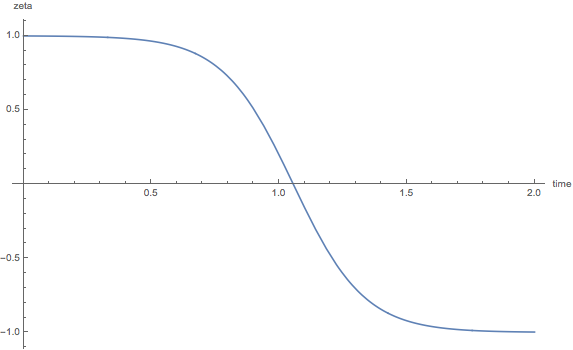
\includegraphics[width=0.5\textwidth]{Images/NeoclassicalDecay.png}
%   \caption{Non-exponential decay of $\zeta$, $\frac{g}{\kappa} = 50, \zeta(0) \approx 1$} \label{fig:neoclassical}
% \end{figure}
\subsubsection{Steady State}
We now set all derivatives to zero, and consider the asymptotic solutions to the mean-field equations, which must satisfy:
\begin{align}
  -ig \beta -i \Epsilon &= 0 \\
  ig\alpha \zeta &= 0
\end{align}
from which are obvious two branches of solutions $\rightarrow \zeta = 0$ or $\alpha = 0$. We take $\alpha = 0$ and from \cref{eq:alpha} and \cref{eq:pseudospin}
\begin{align}
  \beta &= -\frac{\Epsilon}{g} \\
  \zeta &= \mp \sqrt{1 - {\left( \frac{2\Epsilon}{g} \right)}^2}
\end{align}
Increasing drive through the critical point $\Epsilon = \frac{g}{2}$ the difference under the square root becomes negative and the inversion $\zeta$ imaginary and unphysical. We take up the other branch $\zeta = 0$, and from \cref{eq:alpha}
\begin{align}
  \beta &= \pm \frac{\alpha}{2|\alpha|} \\
  \zeta &= 0
\end{align}
with $\alpha$ a solution to
\begin{equation}
  \alpha = -i \Epsilon{\left ( \kappa \pm i \frac{g}{2|\alpha|} \right )}^{-1}
  \label{eq:alphacondnotdet}
\end{equation}

\begin{figure}[h]
  \begin{minipage}{.5\linewidth}
    \centering
    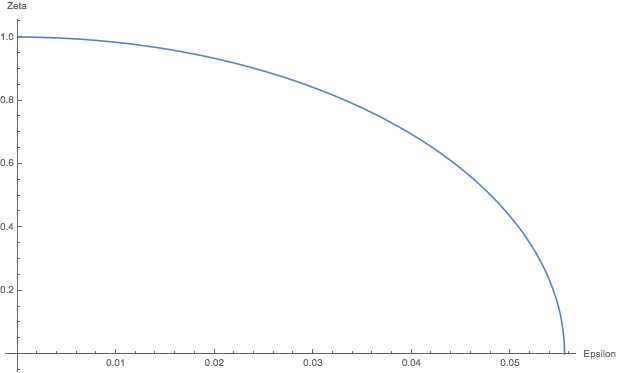
\includegraphics[width=1\textwidth]{Images/MeanFieldBelowCritical.png}
    \caption{$\zeta$ approaches zero with increasing drive strength (positive branch)}\label{fig:zeta}
  \end{minipage}%
  \begin{minipage}{.5\linewidth}
    \centering
    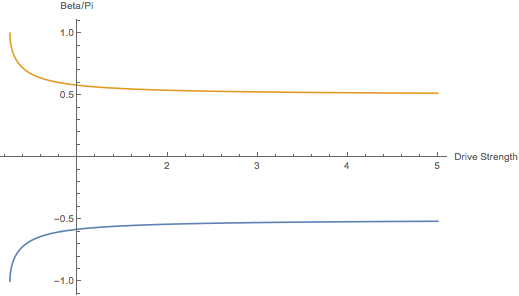
\includegraphics[width=1\textwidth]{Images/MeanFieldAboveCritical.png}
    \caption{Phase of $\beta$ with increasing drive greater than critical}\label{fig:alpha}
  \end{minipage}
  \caption{$\alpha$ and $\zeta$ as the drive strength $\Epsilon$ moves up to through and beyond the critical point}
\end{figure}

in \cref{fig:alpha} the phase bistability above the critical point is obvious. The two $\beta$ solution branches start coincident in phase ($\pi$ and $-\pi$) at drive strengths just above critical and quickly move to opposite sides of the Bloch sphere ($-\frac{\pi}{2}$ and $\frac{\pi}{2}$).

The phase of $\beta$ above the critical point follows the phase of $\alpha$, either aligned or antialigned. This spontaneous development of phase bistability Alsing and Carmichael call `Spontaneous Dressed State Polarisation' \cite{Alsing1990}. Referred to the fully quantum model, each of the two phases corresponds to a the system ascending different sets of rungs of the Jaynes Cummings ladder, either $\ket{E_{n, U}}$ or $\ket{E_{n, L}}$
\subsubsection{Non-zero detuning}
Solving \cref{eq:alpha}, \cref{eq:beta}, \cref{eq:zeta} in the steady state gives
\begin{align}
  \alpha& = i \Epsilon\frac{1}{[\kappa-i(\Delta \omega \mp sgn(\Delta \omega) \frac{g^2}{\sqrt{\Delta \omega^2 +4g^2 |\alpha|^2}})]}
\end{align}
as a condition that $\alpha$ should satisfy, and
\begin{align}
  \beta& = \pm sgn(\Delta \omega) \frac{g \alpha}{\sqrt{\Delta \omega^2 + 4 g^2 |\alpha|^2}}\\
  \zeta& = \mp \sqrt{1-4|\beta|^2}
\end{align}
for $\beta$ and $\zeta$, where $sgn(\Delta \omega)$ is the sign of the detuning with $sgn(0) = 1$.

The expression for $\alpha$ is a Lorentzian, in which is obvious a nonlinear dispersion which diverges as $|\alpha|^2 \rightarrow 0$

A surface plot of $|\alpha|^2 \approx n$ is shown in \ref{fig:MeanFieldvsQuantum}.
\subsection{Numerics}
\begin{figure*}
 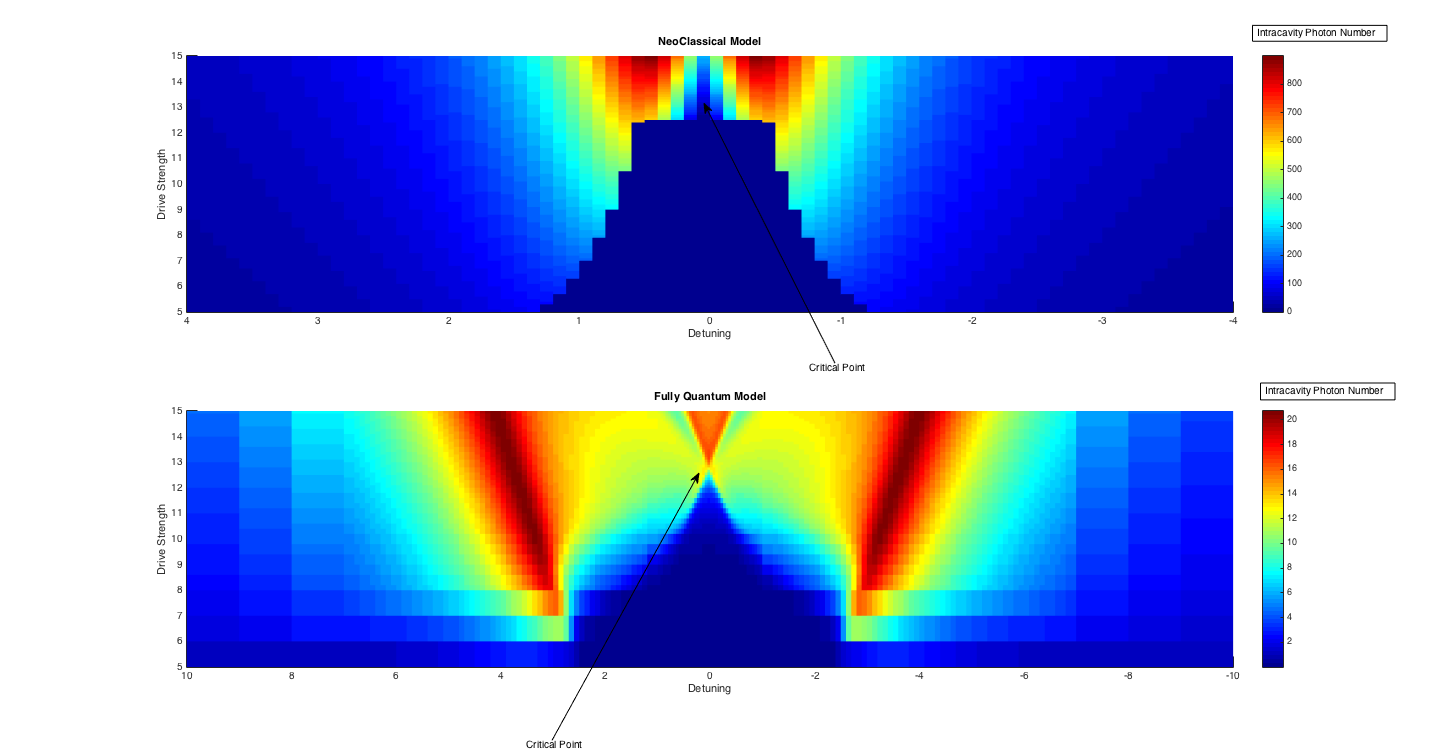
\includegraphics[width=\textwidth]{Images/MeanFieldvsQuantum.png}
 \caption{Comparison of mean field and fully quantum contour plots with critical points at $\frac{\Epsilon}{2}$ highlighted}\label{fig:MeanFieldvsQuantum}
 \end{figure*}

Truncating the master equation density matrix Fock state expansion produces a finite set of coupled differential equations for the components, from which for low photon occupation expectation values in full quantum generality can be generated to high accuracy. This method does however scale incredible poorly in the system size (the number of elements in the density matrix $\propto N^2$, where N is the dimension of the system Hilbert space. The method of quantum trajectories scales much better \cite{Molmer1993} $\propto N$ by considering the wavefunction stochastically). Setting the time derivatives to zero here yields a matrix equation, which given the positive definiteness and hermiticity conditions on the density matrix yields to a Cholesky solver \cite{Press1992}. We use the Matlab and Python solvers as exposed by QuTiP \cite{Johansson2013a} and qotoolbox\cite{Tan1999a}. For the time dependent solutions, we also use fourth order runge-kutta methods provided in both libaries.

The multiple peaks in the bilorentzian (at the bottom of \cite[Figure 1]{Carmichael2015}) as we move from large to little detuning are a mark of multiphoton blockades and their breaking through.

The sides of the Lorentzians correspond to domains of coexistence between the near vacuum state and the high occupation state \cite{Carmichael2015}, and the phase transition between the two at this boundary is of first order, its discontinuity relating to the breaking down of blockade. The transition as the drive strength moves through the critical point is of second order, as indicated in the plots of the approach to equilibrium below, where critical slowing in the approach close to the critical point reveals its nature.

All such features are obvious in our plots in \cref{fig:MeanFieldvsQuantum}, where the quantum results in \cite{Carmichael2015} have been reproduced. Computationally solving the for $\alpha$ in the meanfield condition above yields the first plot.

Numerical calculation of the Q function along the walls of the bilorentzian show a marked bimodality in amplitudeThe development of this Q function bimodality is echoed in the Wigner representation, and is clear in \cref{fig:Qbistabilities}, although the parameters are different to those in \cref{fig:MeanFieldvsQuantum} and in \cite{Carmichael2015}. Moving through the critical point in the drive, the Q function bifurcates, this time in phase, where two coexistent gaussian peaks in phase space mark the phase bistability discussed above.
\begin{figure}
 \begin{minipage}{.5\linewidth}
  \centering
  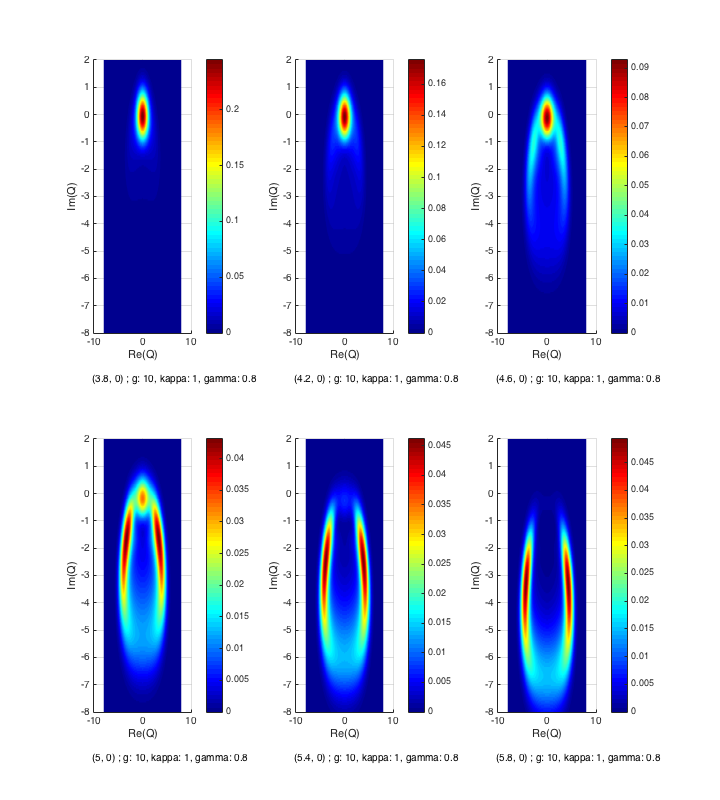
\includegraphics[width=1\textwidth]{Images/Q-Bistability-OnResonance.png}
  \caption{Development of phase bistability in the W function for fixed detuning, with drive moving through the critical point at $\frac{\Epsilon}{2}$}
  \end{minipage}%
  \begin{minipage}{.5\linewidth}
      \centering
      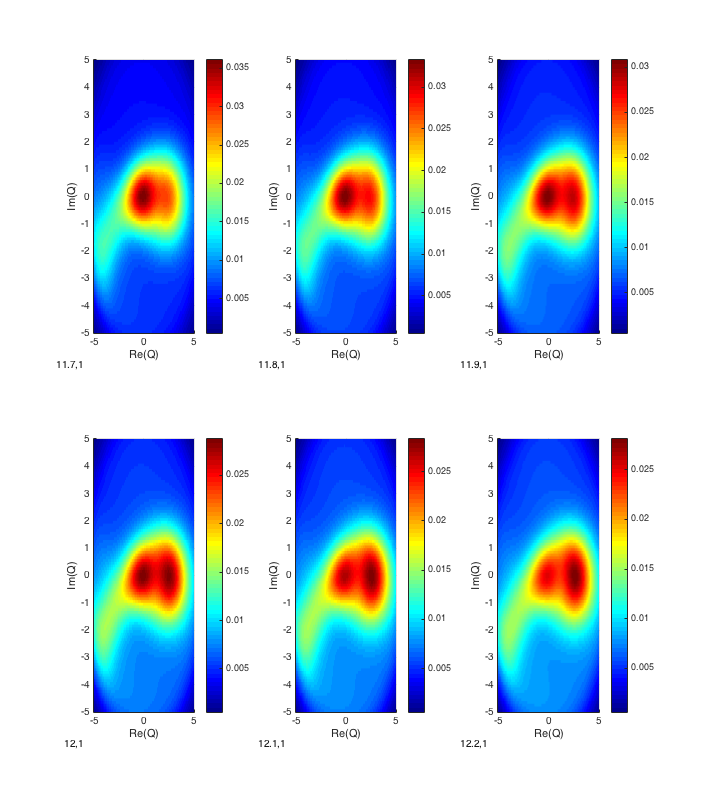
\includegraphics[width=1\textwidth]{Images/Q-Bistability.png}
      \caption{W functions with changing detuning and fixed drive. Note the probability fringes to the right connecting the peaks by spontaneous emission}
  \end{minipage}
  \caption{Q-bistabilities}\label{fig:Qbistabilities}
\end{figure}

\begin{figure*}
  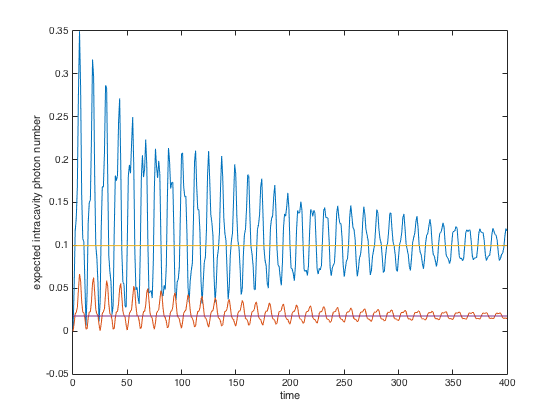
\includegraphics[width=\textwidth]{Images/CriticalSlowing.png}
  \caption{Time Dependent Solutions with g=0.5, $\kappa$ = 0.01, blue line is (0.24, 1), red line is (0.1, 1)}\label{fig:CriticalSlowing}
\end{figure*}

\subsection{Spontaneous Emission}.

We now reintroduce the spontaneous emission parameter, both in the mean-field and the quantum case. In \ref{fig:Qbistabilities} we show Q functions along the inner walls of the bilorentzian in \ref{fig:MeanFieldvsQuantum} and through the critical point in the drive, with the spontaneous emission parameter present.

Deexcitation fringes are clear in \ref{fig:Qbistabilities} where a spontaneous emission rate $ \gamma = \frac{\kappa}{2}$ connects the peaks of both of the bistabilities: in phase and in amplitude. Given the interpretation of such bimodal quasi-probability functions in the zero detuning case as as having a probability peak for the occupation of each ladder, it is clear that spontaneous emission serves to induce ladder-switching. It is this ladder switching that washes out the semiclassical bistability in the quantum regime.

We return to mean-field equations. The optical Bloch equations with spontaneous emission read:
\begin{align}
\frac{d \alpha}{dt} &= -(\kappa - i \Delta \omega)\alpha - ig \beta - i\Epsilon\label{eq:alphase}\\
\frac{d \beta}{dt} &= -(\frac{\gamma}{2}-i\Delta\omega)\beta+ig\alpha\zeta \label{eq:betase}\\
\frac{d\zeta}{dt} &= -\gamma (\zeta +1)+2ig(\alpha^*\beta-\alpha\beta^*) \label{eq:zetase}
\end{align}
In the steady state \cref{eq:alphase} becomes
\begin{align}
  \beta &= \frac{ig\alpha\zeta}{\frac{\gamma}{2}-i\Delta\omega}
\end{align}
from which in \cref{eq:zetase} in steady-state
\begin{align}
  0 &= -\gamma(\zeta+1)+2ig\frac{ig|\alpha|^2\zeta\frac{\gamma}{2}2}{\frac{\gamma^2}{4}+\Delta\omega^2} \\
  \implies \zeta &= \frac{1}{\frac{-2g^2|\alpha|^2}{\frac{\gamma^2}{4} +\Delta\omega^2}-1} \\
  &= \frac{1}{\frac{-2g^2|\alpha|^2 - \frac{\gamma^2}{4}-\Delta\omega^2}{\frac{\gamma^2}{4} +\Delta\omega^2}}
\end{align}
putting the above together yields
\begin{align}
  \beta &= \frac{ig\alpha\zeta}{\frac{\gamma}{2}-i\Delta\omega}\\
  &= \frac{ig\alpha}{\frac{(-2g^2|\alpha|^2-\frac{\gamma^2}{4}-\Delta\omega^2)(\frac{\gamma}{2}-i\Delta\omega)}{\frac{\gamma^2}{4}+\Delta\omega^2}}\\
  &= \frac{ig\alpha}{\frac{-2g^2|\alpha|^2-\frac{\gamma^2}{4}-\Delta\omega^2}{\frac{\gamma}{2}+i\Delta\omega^2}}\\
  &= \frac{ig\alpha(\frac{\gamma}{2}+i\Delta\omega)}{-2g^2|\alpha|^2-\frac{\gamma^2}{4}-\Delta\omega^2} \label{eq:betasolved}
\end{align}
\cref{eq:alphase} in the steady state with  \cref{eq:betasolved} becomes a condition for $\alpha$
\begin{align} % Here be weird bugs
0&=-(\kappa-i\Delta\omega)\alpha-ig\beta-i\Epsilon \\
0&=-{(\kappa-i\Delta\omega)}\alpha-g\frac{ig(\frac{\gamma}{2}+i\Delta\omega)}{-2g^2|\alpha|^2-\frac{\gamma^2}{4}-\Delta\omega^2}\alpha-i\Epsilon \\
\implies \alpha &= -i\Epsilon \frac{1}{\kappa-i\Delta\omega+\frac{g^2(\frac{\gamma}{2}+i\Delta\omega)}{\frac{\gamma^2}{4}+{\Delta\omega}^2+2g{|\alpha|}^2}}\label{eq:alphadetdiss}
\end{align}
Setting $\gamma$ and $\Delta\omega$ to zero, the condition becomes
\begin{equation}
  \alpha = -i\Epsilon\frac{1}{\kappa}
\end{equation}
which is notably not the same as \cref{eq:alphacondnotdet}.

\subsubsection{Difference between limits}\cite{Alsing1990}
  The presence of $\gamma$ in the Maxwell-Bloch Equations changes the asymptotic solutions, even if $\gamma$ is set to zero in these solutions. This is down to the breaking of the conservation law $4|\beta|^2 +\zeta^2 = 1$ by the presence of spontaneous emission. The solutions in the case that the limit is taken after steady state requirement is imposed are those of absorptive optical bistability. In the limit $\frac{\gamma}{\kappa} \rightarrow 0$ the rate at which these steady states becomes vanishingly small

\Cref{eq:alphadetdiss} is the classical solution for the steady state of a saturable two level transition, with a saturation photon number ($I \propto |\alpha|^2 \approx n_{sat}$) of $n_{sat} = \frac{\gamma^2}{8g^2}$.

\subsection{Dispersion}
We now move to the dispersive regime, where the cavity qubit detuning $\delta_{cq}$ is very large compared to the other frequencies in the problem. Following the work of Ginossar and Bishop \cite{Bishop2010}, we build a semiclassical model for the system
\begin{equation}
\mathscr{H} = \omega_c \cre \ann + ( \omega_c - \Delta ) \sigma_z /2 + \frac{\chi}{\sqrt{2}} (\ann + \cre ) cos(\omega_d t)
\end{equation}
which is solvable but for the term $\Delta$, defined
\begin{equation}
        \Delta = \sqrt{\delta^2 +4 g ^2 N}
\end{equation}
In which the operator $N = \cre \ann $ appears non-trivially. Rewriting the hamiltonian in terms of the generalised coordinates
\begin{equation}
        \mathscr{H} = \omega_c/1 (X^2 + P^2 + \sigma_z) + \xi X cos(\omega_d t) - \sigma_z /2 \sqrt{2g^2(X^2+P^2+\sigma_z) + \delta^2}
\end{equation}
where the $\delta$ term has been split. We make the semiclassical approximation by treating P and X as numbers, and make the claim that such an assumption holds for all N (intracavity photon number) much greater than $N_{crit}$, where $N_{crit}$ is equal to $\frac{\delta^2}{g^2}$.
From Hamilton's equations for the (semi-) classical Hamiltonian
\begin{align}
        \frac{d\mathscr{H}}{dX} &= \frac{dP}{dt}\\
        \frac{d\mathscr{H}}{dP} &= -\frac{dX}{dt}
\end{align}
in the steady state, setting the second derivatives of the quadratures X \& P to zero and solving for the amplitude $A = X^1 + P^2$, we find
\begin{equation}
        A^2 = \frac{\omega_d^2\xi}{\{\omega_d^2 - [\omega_c - \chi (A) ]^2 \}^2+ \kappa^2 \omega_d^2}
\end{equation}
where
\begin{equation}
        \chi(A) = \sigma_z \frac{g^2}{\sqrt{2g^2(A^2 + \sigma_z) + \delta^2}}
\end{equation}
inverting the equation and solving for $\xi$ as a function of $A^2$, we retrieve for the amplitude as a function of the detuning and the drive strength:
\begin{figure*}
        \includegraphics[width=\textwidth]{Images/SemiclassicalBistability.png}
        \caption{Semiclassical Amplitude as a function of drive and detuning}
\end{figure*}
Areas where the amplitude is not 1-1 (for given drive) indicate the existence of bistability, where the negative gradient intermediate state is metastable, and the system is stable along the upper and lower curves. These regions in the quantum case are washed out by switching induced by quantum fluctuations, and the amplitude in the quantum case can be qualitatively expected to 'average out' the bistability and lie between the two stable states on this plot. Indeed, this effect is visible in the next plot. We see more interesting features here too, most notably a dip in the quantum amplitude, where there is destructive interference between the two stable paths. In a sense, the quantum amplitude is characterised by the switching rate, where at a given detuning, the upwards switching drags the curve upwards and the downwards downwards.
